% !TeX program = xelatex
% Narrative is editable here; numbers.tex and figures are generated from evidence.
\documentclass[10pt,a4paper,twocolumn]{article}
\usepackage{fontspec}
\IfFontExistsTF{Times New Roman}{\setmainfont{Times New Roman}}{\setmainfont{Libertinus Serif}}
\IfFontExistsTF{Arial}{\setsansfont{Arial}}{\setsansfont{DejaVu Sans}}
\IfFontExistsTF{Consolas}{\setmonofont{Consolas}}{\setmonofont{Latin Modern Mono}}
\usepackage[russian]{babel}
\usepackage[margin=18mm,top=19mm,bottom=19mm,footskip=9mm]{geometry}
\usepackage{amsmath,amssymb,booktabs,array,microtype,graphicx,xcolor}
\usepackage{titlesec,fancyhdr,balance}
\usepackage[font=small,labelfont={bf,sf},labelsep=period]{caption}
\usepackage[colorlinks=true,linkcolor=black,urlcolor=teal,citecolor=teal]{hyperref}
\definecolor{ink}{HTML}{243747}
\definecolor{teal}{HTML}{176C79}
\definecolor{muted}{HTML}{657785}
\setlength{\columnsep}{7mm}
\setlength{\parindent}{.8em}
\setlength{\parskip}{1.5pt}
\setlength{\textfloatsep}{10pt}
\setlength{\dbltextfloatsep}{12pt}
\setlength{\headheight}{14pt}
\emergencystretch=2em
\clubpenalty=10000\widowpenalty=10000\displaywidowpenalty=10000
\vfuzz=2pt
\titleformat{\section}{\sffamily\bfseries\fontsize{11}{13}\selectfont\color{ink}}{\thesection}{.6em}{}
\titlespacing*{\section}{0pt}{9pt}{4pt}
\titleformat{\subsection}{\sffamily\bfseries\fontsize{9.5}{11.5}\selectfont}{\thesubsection}{.5em}{}
\titlespacing*{\subsection}{0pt}{6pt}{3pt}
\pagestyle{fancy}\fancyhf{}
\fancyhead[L]{\sffamily\fontsize{7}{8}\selectfont\color{muted}RL В ПОСЛЕДОВАТЕЛЬНЫХ РЕКОМЕНДАЦИЯХ}
\fancyhead[R]{\sffamily\fontsize{7}{8}\selectfont\color{muted}YAMBDA / GPT-2}
\fancyfoot[C]{\sffamily\small\thepage}
\renewcommand{\headrulewidth}{.25pt}
\raggedbottom
% Generated from reports/task2/evidence; edit narrative in article.tex.
\newcommand{\EvalUsers}{266}
\newcommand{\EvalQueries}{2770}
\newcommand{\CatalogCoverage}{52.6}
\newcommand{\MacroCeiling}{0.5433}
\newcommand{\PrimaryDelta}{-0.000037}
\newcommand{\PrimaryLo}{-0.000571}
\newcommand{\PrimaryHi}{+0.000497}
\newcommand{\SftNdcg}{0.01097}
\newcommand{\RepeatNdcg}{0.01153}
\newcommand{\ProxyBefore}{0.7143}
\newcommand{\ProxyAfter}{0.7242}
\newcommand{\FitCount}{48}
\newcommand{\FitMinutes}{9.6}
\newcommand{\MainRows}{%
Popularity & 0.00198 & 0.00486 & 0.00111 \\
Markov & 0.00638 & 0.01153 & 0.00485 \\
Repeat & 0.01153 & 0.01867 & 0.00938 \\
GPT-2 / CE & 0.01097 & 0.02134 & 0.00794 \\
+ CE & 0.01131 & 0.02189 & 0.00820 \\
Ratio & 0.01102 & 0.02092 & 0.00807 \\
Seconds & 0.01102 & 0.02154 & 0.00797 \\
Activity & 0.01085 & 0.02063 & 0.00797 \\
Ensemble H=1 & 0.01072 & 0.02115 & 0.00767 \\
Ensemble & 0.01117 & 0.02167 & 0.00804 \\
Anchored & 0.01113 & 0.02067 & 0.00828 \\
}
\newcommand{\RewardRows}{%
Global mean & 0.1806 & 0.3777 & 0.500 & 0.1359 \\
Item mean & 0.1813 & 0.3743 & 0.525 & 0.1363 \\
Ensemble RM & 0.1798 & 0.3496 & 0.568 & 0.1379 \\
Audit RM & 0.1834 & 0.3521 & 0.581 & 0.1396 \\
Чужая история & 0.2056 & 0.3801 & 0.488 & 0.1453 \\
}


\begin{document}
\twocolumn[{
\begin{center}
{\sffamily\bfseries\fontsize{19}{22}\selectfont\color{ink}
Оптимизация выученной награды\\в последовательных рекомендациях\par}
\vspace{5pt}
{\sffamily\fontsize{10}{12}\selectfont GPT-2, пять шагов генерации и контроль вымышленной истории\par}
\vspace{5pt}
{\sffamily\fontsize{8}{10}\selectfont\color{muted}Воспроизводимое исследование на Yambda 50M \enspace / \enspace Октябрь 2026\par}
\end{center}
\vspace{3pt}
\noindent\textbf{Аннотация.}
Можно ли повысить предсказанную награду рекомендаций, сохранив их точность?
Мы обучили GPT-2 на идентификаторах треков и дообучили её с помощью REINFORCE
по модели отклика. Исследованы пять наград и три силы KL-штрафа.
В отдельной когорте из \EvalUsers{} активных пользователей ансамблевая награда
повысила оценку доли прослушивания с \ProxyBefore{} до \ProxyAfter{},
но прирост NDCG@10 не подтверждён. Предложенный штраф за расхождение
оценки в реальной и дополненной истории также не дал убедительного выигрыша:
$\Delta=\PrimaryDelta$, 95\% интервал $[\PrimaryLo;\PrimaryHi]$.
Пятишаговый аудит показывает, как добавление собственных рекомендаций в контекст
повышает оценку reward model без наблюдения пользовательской реакции.
\vspace{10pt}
}]

\section{Проблема и проверяемая идея}

Последовательная модель воспроизводит следующее действие из лога.
RL меняет цель, например на долю прослушивания или последующую активность.
Настоящий отклик на новый выбор неизвестен: оптимизатор может улучшать
прогноз модели отклика, а не пользовательский опыт.

При генерации пяти треков каждый выбранный ID добавляется в контекст.
Но рекомендация ещё не означает прослушивание. RM оценивает кандидата
по истории, содержащей неподтверждённые действия.

Мы оцениваем один кандидат в дополненной истории $h_t$ и исходной
реальной истории $h_0$, затем штрафуем расхождение. Контроль с той же
ансамблевой наградой изолирует добавленный штраф. Это экспериментальная
гипотеза без заявления мирового приоритета или теоретической гарантии.

\section{Данные и честная оценка}

Использована таблица \texttt{listens} Yambda 50M, pinned revision из
репозитория. Из пользователей двух предыдущих исследований исключены
все UID; затем равномерно выбраны 1200 новых пользователей.
Сохранены все 5\,736\,029 исходных строк выбранных UID, включая короткие
прослушивания и органические действия. Sampling seed~718281;
разбиение UID на development~800 / external~400 зафиксировано до обучения.

Время анонимизировано: сутки равны~86\,400 секундам.
Модели обучаются на событиях до day~270; подбор настроек использует
days280--286 только development UID. Внешняя оценка проводится на
days293--298 только external UID. Их ранние истории участвуют в обучении,
но поздние метки не выбирают настройки. Это временной holdout с другой
когортой оценки, а не cold-user задача или независимая будущая репликация:
период частично совпадает с первой работой, пользователи не пересекаются.

Каждый запрос предсказывает один следующий неорганический listen.
Оцениваются первые до четырёх событий с уникальным timestamp за user-day.
Нет отбора по доле прослушивания. История содержит только события
строго раньше запроса. Переходы между строками с одинаковым timestamp
не входят в supervised loss; их искусственный порядок не считается
известной последовательностью действий.

Каталог всех методов одинаков: 16\,384 самых частых train items.
Повторы разрешены. Будущая цель не добавляется в каталог.
По числу запросов вне словаря осталось~47.4\% внешних целей;
они остаются промахами в знаменателях. Это существенное ограничение
бюджета, а не только cold-start: вне словаря бывают и редкие старые треки.
Максимально возможный user-macro Recall для этого каталога равен
\MacroCeiling{}. Истории сохраняются полностью; модельный контекст
ограничен последними~64 ID, неизвестные ID кодируются UNK.

На внешнем периоде получены \EvalQueries{} запроса от \EvalUsers{} активных
тёплых пользователей. NDCG, Recall и MAP при $K=10$ сначала усредняются
по трём model seeds для запроса, затем по запросам внутри пользователя
и по пользователям. Интервалы разностей получены парным bootstrap
целых пользователей, 3000 resamples. Они условны на этих данных и fits;
не покрывают другие периоды и весь риск выбора настроек.

\section{Модели и обучение}

\subsection{GPT-2 и простые контроли}
Используется уменьшенная архитектура GPT-2 с нуля: learned item и position
embeddings, три pre-LN causal decoder блока, размерность~128, четыре heads,
GELU, MLP expansion4, final LayerNorm и общий вес input/output embeddings.
Всего~2.70 млн параметров. Это модель над item IDs; текстовые pretrained
weights не используются. Полная softmax рассчитывается по всему каталогу.
Исходную обученную модель обозначаем SFT.

Первоначальный бюджет~1500 updates дал development NDCG~0.00958.
До открытия внешнего теста он был увеличен до~12\,000: лучший checkpoint
на development оказался на~3000 updates, NDCG~0.01453. Дальнейшее
снижение train loss не улучшило ranking. Поправка протокола,
полная траектория и девять пилотных RL fits сохранены.

AdamW: lr$=3\cdot10^{-4}$, weight decay~0.01, warmup~300,
cosine schedule до~12\,000, effective batch~64. Seeds~17/42/73
получают одинаковые~3000 выбранных updates; seed~17 также несёт цену
полного checkpoint search. Контроли используют тот же каталог:
train popularity, повторное потребление по доступному контексту,
Markov первого порядка со сглаживанием popularity. Дополнительный
CE fit на~120 updates проверяет пользу продолжения supervised обучения;
он не является joint NLL+RL baseline.

\subsection{Модель отклика}
RM получает историю ID и ID кандидата. Отдельные embeddings
позволяют вычислить mean/last history pooling и взаимодействие
истории с кандидатом; к MLP добавлена статическая длительность
из train. Текущий played ratio не входит во вход модели.
Две sigmoid heads предсказывают:
(1) $y=\min(1,\texttt{played\_ratio\_pct}/100)$;
(2) наличие события в $[t+1\mathrm{h},t+24\mathrm{h})$.
Второй сигнал обозначаем \emph{Activity}. Он описывает последующую
активность, включая продолжающееся потребление, а не доказанный возврат
после ухода из сервиса.

RM обучается только на реально наблюдавшихся неорганических listens
до day~269: её 24h label horizon целиком заканчивается до day~270.
Неизвестные отклики на непрослушанные кандидаты не размечаются нулями.
До~1500 train examples на пользователя, всего~855\,792;
batch~512, lr$=10^{-3}$, 800 updates, fractional/binary BCE.
Три RM с seeds~17/42/73 образуют ансамбль. Четвёртая, audit RM seed~101,
не участвует в reward; она имеет другую инициализацию, но те же данные
и архитектуру. Она не является независимой разметкой или oracle.

\subsection{Награда и policy gradient}
Пусть $m(h,a)$ и $s(h,a)$ --- среднее и population std трёх ratio heads.
Сравниваются пять наград: Ratio (одна RM), Seconds
($\hat y\min(d,600)/600$), Activity ($0.5\hat y+0.5\hat p_{24}$),
а также два контролируемых варианта:
\begin{align}
r_E(h_t,a)&=m(h_t,a)-0.5s(h_t,a),\\
r_A(h_t,a)&=r_E(h_t,a)-|m(h_t,a)-m(h_0,a)|.
\end{align}
Разброс ансамбля не считается калиброванной неопределённостью.
Последний штраф нулевой на первом шаге. Он может подавлять и полезный
контекстный сдвиг, поэтому его эффект требует проверки.

REINFORCE запускается \emph{on-policy внутри выученного surrogate},
не в настоящей пользовательской среде. Каждый rollout начинается
с реального train prefix, пользователь выбирается равномерно.
Пять раз сэмплируется ID из полной softmax; ID добавляется в контекст,
выдуманные playback labels не добавляются. Награда регуляризуется
относительно замороженной SFT policy $\pi_0$:
\begin{align}
\widetilde r_t&=r_t-\beta\log\frac{\pi_\theta(a_t\mid h_t)}{\pi_0(a_t\mid h_t)},\\
G_t&=\sum_{j=t}^{H-1}\gamma^{j-t}\widetilde r_j.
\end{align}
Градиент использует $\gamma^t(G_t-b_t)\nabla\log\pi_\theta(a_t\mid h_t)$;
baseline $b_t$ --- среднее return других независимых trajectories batch.
Dropout у policy выключен. AdamW lr$=5\cdot10^{-5}$,
$\gamma=0.9$, batch~96, 120 updates, grad clip1.

На development проверены $5\times3=15$ конфигураций,
$\beta\in\{0.02,0.1,0.5\}$. В каждой семье выбиралась наибольшая
предсказанная доля среди точек с NDCG не ниже~95\% SFT.
Это правило выбора, а не статистическое доказательство non-inferiority.
Выбраны $\beta=0.1$ для Ratio/Ensemble/Anchored и~0.5 для Seconds/Activity.
Главное заранее заданное сравнение --- Anchored$-$Ensemble при
одинаковом $\beta=0.1$. Контроль $H=1$ имеет те же~120 updates,
но в пять раз меньше sampled actions: это ограничение его интерпретации.

\begin{table}[t]
\centering\small
\caption{Внешнее качество следующего logged item. Среднее отдельных
fits seeds~17/42/73, а не ансамбль policy. Лучший простой контроль
обязателен для интерпретации; point estimate не равен значимому выигрышу.}
\label{tab:main}
\begin{tabular}{lrrr}\toprule
Метод & NDCG@10 & Recall@10 & MAP@10\\\midrule
\MainRows
\bottomrule\end{tabular}
\end{table}

\begin{figure*}[t]
\centering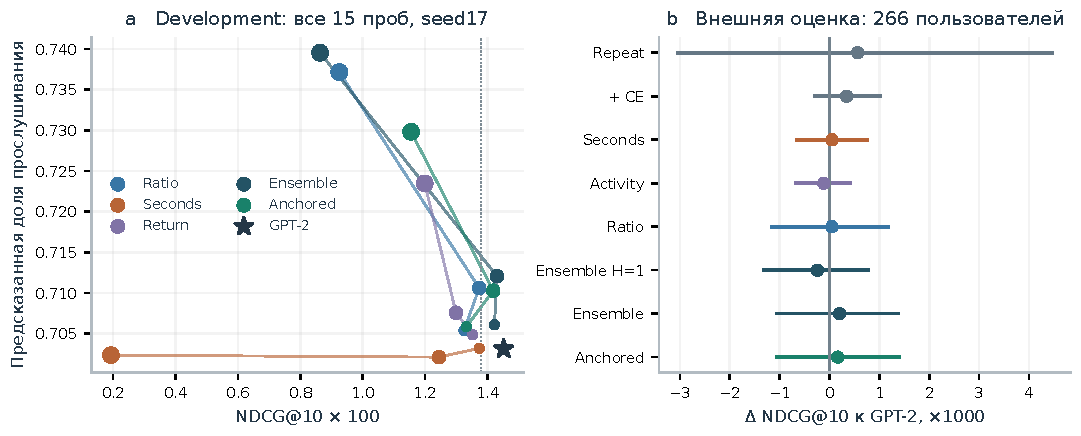
\includegraphics[width=\textwidth]{figures/tradeoff.pdf}
\caption{Слева --- полный development search. Общая вертикальная ось
показывает ratio RM и для политик с другими rewards; размер точки растёт
при уменьшении $\beta$ (0.5,0.1,0.02). Пунктир --- правило~95\% SFT.
Справа --- внешние разности с SFT и описательные~95\% user-cluster CI.
Ни один RL-вариант не подтвердил прирост NDCG. Это не доказательство эквивалентности.}
\label{fig:tradeoff}
\end{figure*}

\section{Результаты и причины}

\subsection{Релевантность и цена награды}
Внешняя SFT получила NDCG~\SftNdcg{}, Repeat --- \RepeatNdcg{}.
Разность Repeat$-$SFT~0.00057 имеет интервал
$[-0.00305;0.00446]$: превосходство простого контроля также не установлено.
Абсолютные числа нельзя сравнивать с первой задачей: там предсказывалось
множество треков за сутки, здесь --- одно следующее действие.

Ensemble повышает предсказанную ratio top1 с~\ProxyBefore{}
до~\ProxyAfter{}. NDCG растёт лишь на~0.00020,
CI$[-0.00105;0.00138]$. Все выбранные RL-варианты имеют интервалы
к SFT, включающие ноль (рис.~\ref{fig:tradeoff}). Доказательств
улучшения реальной релевантности нет. Разброс seed заметен:
для Ensemble NDCG составляет 0.01248/0.01025/0.01077.

Основной контраст Anchored$-$Ensemble:
$\PrimaryDelta$, CI$[\PrimaryLo;\PrimaryHi]$.
Штраф не подтвердил преимущество. Он уменьшил среднюю exact KL
с~0.1145 до~0.0979, но само по себе меньшее отклонение от SFT
не является улучшением рекомендаций.

Смена награды меняет состав выдачи предсказуемым способом.
Ratio рекомендует в среднем~182 секунды против~192 у SFT;
Seconds ---199 секунд. На development слабый KL у Seconds
($\beta=0.02$) увеличил среднюю длительность до~390 секунд,
один трек занял~51.3\% top1, NDCG упала до~0.00193.
Эта точка не выбрана и не выдаётся за внешний результат.
В выбранных внешних точках такого коллапса нет:
самый частый top1 занимает около~1--2\% запросов.

\subsection{Насколько надёжна RM}
Таблица~\ref{tab:reward} показывает метрики на всех внешних logged actions,
включая цели вне каталога. MSE/MAE здесь усредняются по событиям;
их bootstrap сохраняет кластеры пользователей.
Ансамбль едва превосходит постоянное среднее по ratio MSE:
0.1798 против~0.1806; по индивидуальным RM ошибка хуже.
Надёжное улучшение MSE не подтверждено
(рис.~\ref{fig:reward},b). При этом MAE ниже, а подмена пользовательской
истории чужой доступной историей повышает MSE до~0.2056.
Следовательно, модель использует соответствие контекста пользователю,
но это не обеспечивает точность всех условных прогнозов.

Activity AUC ансамбля~0.568 показывает слабое различение будущей
активности. Её Brier~0.1379 хуже константы~0.1359.
Увеличение такого reward нельзя интерпретировать как улучшение удержания.
Согласие audit RM с оптимизируемой RM также не заменяет
контрфактуальную разметку: общие данные создают общие ошибки.

\begin{table}[t]
\centering\small\setlength{\tabcolsep}{3pt}
\caption{RM на~2770 реально наблюдавшихся действиях. Ratio MSE/MAE;
AUC и Brier относятся к Activity. «Чужая история» --- диагностическая
подмена контекста при неизменном кандидате, а не новая обученная модель.}
\label{tab:reward}
\begin{tabular}{lrrrr}\toprule
Модель & MSE & MAE & AUC & Brier\\\midrule
\RewardRows
\bottomrule\end{tabular}
\end{table}

\begin{figure*}[t]
\centering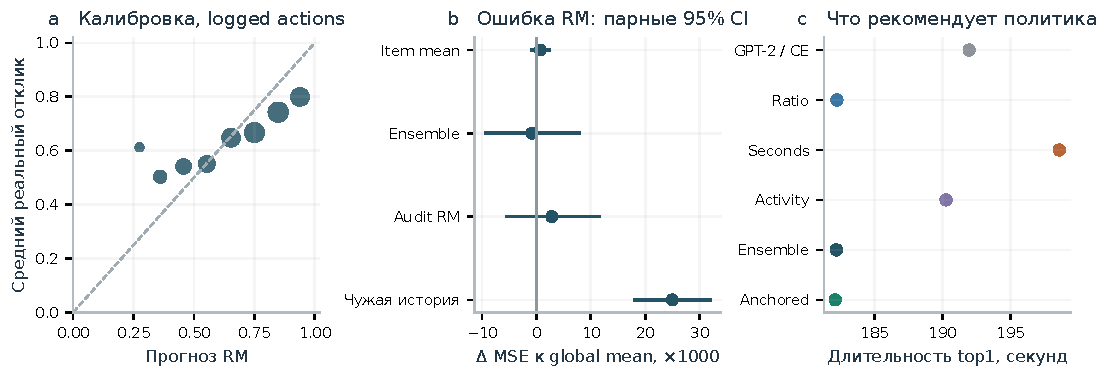
\includegraphics[width=\textwidth]{figures/reward_audit.pdf}
\caption{Аудит RM и политики. В калибровке размер точки пропорционален
корню из числа примеров bin; bins с менее~10 событиями не показаны.
Интервалы MSE получены resampling пользователей с сохранением
взвешивания по событиям. Справа --- длительность рекомендованного top1,
среднее по пользователям и seeds; это не фактическое время прослушивания.}
\label{fig:reward}
\end{figure*}

\subsection{Пять шагов и вымышленная история}
Для~256 пользователей взят один реальный начальный prefix.
Каждая policy генерирует пять actions, отдельно с обновлением контекста
и с замороженной историей. Sampling seeds связаны: первый action
в двух режимах совпадает. Значения на рис.~\ref{fig:rollouts}
описательные, без выбора новых настроек.

В режиме обновления история сама повышает прогноз ratio Ensemble
примерно с~0.717 до~0.737. При замороженной истории оценка остаётся
около~0.718. Но никакой реакции на выбранные треки не наблюдалось.
К пятому шагу средняя абсолютная разница RM для одного action
в дополненном и первоначальном контексте достигает около~0.05.
Anchored не уменьшил этот сдвиг убедительно; его кривая близка
к Ensemble. Повторы внутри списка составляют несколько процентов,
а не объясняют весь рост proxy.

Отдельная teacher-forced проверка использует следующие реальные actions
и настоящие prefixes, а не сгенерированные ID. Число доступных пользователей
уменьшается по шагам; это сохранено в evidence. Уже на первом запросе
каждого пользователя ratio MSE~0.244, хотя по всей внешней выборке~0.180.
У generated actions истинной MSE нет: сравнение их reward с observed
trajectory не оценивает причинный эффект.

\begin{figure*}[t]
\centering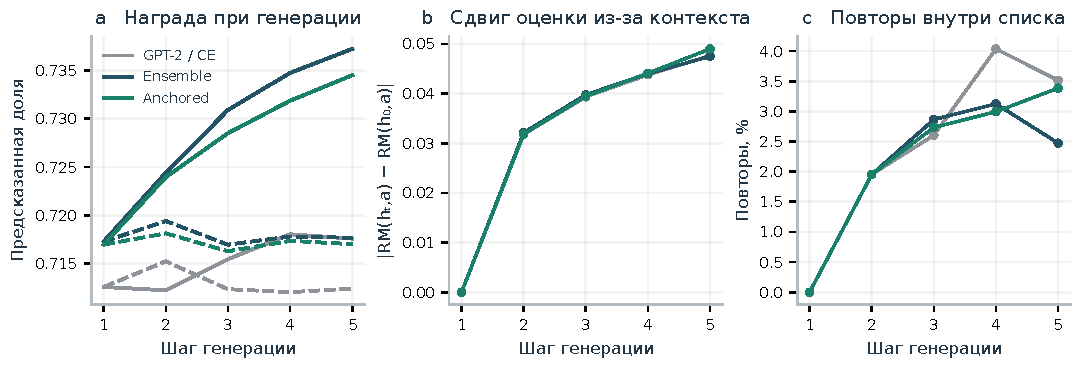
\includegraphics[width=\textwidth]{figures/rollouts.pdf}
\caption{Пятишаговый model-based аудит,256 пользователей, три policy seeds.
Сплошные линии --- generated ID добавляются в историю;
пунктир слева --- та же policy с замороженной историей.
Середина сравнивает один и тот же выбранный action в двух контекстах.
Правый график --- вероятность повторить ранее выбранный в этом списке ID.
Отклики пользователей в этом эксперименте не симулируются как реальные события.}
\label{fig:rollouts}
\end{figure*}

\section{Связь с литературой и ограничения}

GPTRec~\cite{gptrec} использует Next-K генерацию, teacher--student
и PPO; здесь обучается next-item GPT-2~\cite{gpt2} и RM отклика.
В отличие от off-policy REINFORCE на Yambda-5B~\cite{session},
нет известных logging propensities и оценок IPS/DR.
Наши model-based средние не являются unbiased policy value;
цели вне словаря не добавляются в каталог оценки.

Риск overoptimization~\cite{gao} и консервативные ансамбли RM~\cite{coste}
известны. Наш вклад --- отдельная проверка контекстного штрафа
с matched-beta контролем, вместе с диагностикой реальной и вымышленной
истории. Теоретические гарантии MOPO~\cite{mopo} на него не переносятся:
пользовательская transition dynamics не обучается.
AdaGRPO~\cite{adagrpo} мотивирует селективное доверие noisy rewards;
её NLL+GRPO gate здесь не реализован. Это важный недостающий сильный контроль.

Основные ограничения: 1200 пользователей активной популяции, один период,
малый словарь и слабая RM после временного разрыва. Append-ID surrogate
не описывает решение пропустить трек, уйти или вернуться. Три seeds
не заменяют новые данные и online A/B. Продолжение требует нового
внешнего периода, калибровки RM по типам контекста и модели переходов
с наблюдаемым feedback; текущий test уже открыт.

\section{Вывод и воспроизводимость}

RL действительно меняет выдачу и повышает выученную proxy-награду.
В данном эксперименте это не дало подтверждённого выигрыша next-item
релевантности. Предложенная защита от вымышленной истории также не
подтвердила преимущество. Результат --- измеренное расхождение между
оптимизацией RM, точностью по логам и оценкой на дополненном контексте.

Код, два протокола, полный search, отдельные seeds, сырые top10 forecasts
и компактные доказательства находятся в репозитории.
Все~24 нейронных массива top10 воспроизведены точно;64 проверки
замены будущих items не изменили исторический context;
проверено сохранение всех исходных строк выбранных UID.
Зафиксированы \FitCount{} завершённых fits, включая пилот;
сумма записанных fit durations ---\FitMinutes{} минут на RTX4070TiSUPER.
Это не полное время исследования или изолированный benchmark.

Метрики проверяются без Yambda и GPU. Инструкции полного запуска
и проверки ---в \texttt{TASK2\_REPRODUCE.md} репозитория.

\begin{thebibliography}{7}\scriptsize
\setlength{\itemsep}{1pt}\setlength{\parskip}{0pt}
\bibitem{gpt2} Radford et al. Language Models are Unsupervised Multitask Learners. 2019.
\href{https://github.com/openai/gpt-2}{Architecture/code}.
\bibitem{gptrec} Petrov, Macdonald. Aligning GPTRec with Beyond-Accuracy Goals with Reinforcement Learning. GenRec, 2024.
\href{https://arxiv.org/abs/2403.04875}{arXiv:2403.04875}.
\bibitem{session} Matveev et al. Session-Level Optimization for Large-Scale Retrieval using REINFORCE with Multi-Step Off-Policy Correction. 2026.
\href{https://arxiv.org/abs/2607.02818v2}{arXiv:2607.02818v2}.
\bibitem{gao} Gao, Schulman, Hilton. Scaling Laws for Reward Model Overoptimization. 2022.
\href{https://arxiv.org/abs/2210.10760}{arXiv:2210.10760}.
\bibitem{coste} Coste et al. Reward Model Ensembles Help Mitigate Overoptimization. ICLR, 2024.
\href{https://arxiv.org/abs/2310.02743}{arXiv:2310.02743}.
\bibitem{mopo} Yu et al. MOPO: Model-based Offline Policy Optimization. NeurIPS, 2020.
\href{https://arxiv.org/abs/2005.13239}{arXiv:2005.13239}.
\bibitem{adagrpo} Xu et al. Adaptive Loss Balancing for Noise-Robust GRPO in Generative Recommendation. 2026, preprint.
\href{https://arxiv.org/abs/2606.08480}{arXiv:2606.08480}.
\end{thebibliography}
\end{document}
